%----------------------------------------------------------------------------------------
%	PACKAGES AND THEMES
%----------------------------------------------------------------------------------------
\documentclass[aspectratio=169,xcolor=dvipsnames]{beamer}
\usetheme{Simple}
\usepackage{hyperref}
\usepackage{graphicx} % Allows including images
\usepackage{booktabs} % Allows the use of \toprule, \midrule and \bottomrule in tables
\usepackage{graphicx}
\setbeamertemplate{caption}[numbered]
\setbeamertemplate{footline}[text line]{%
  \parbox{\linewidth}{\vspace*{-8pt}Email:  \href{sanjaykanakkot.viswanathan@gmail.com}{sanjaykanakkot.viswanathan@gmail.com,}    Company Website: \href{https://www.truuth.id}{https://www.truuth.id}\hfill\insertpagenumber}}
   
\setbeamertemplate{navigation symbols}{}

%----------------------------------------------------------------------------------------
%	TITLE PAGE
%----------------------------------------------------------------------------------------

% The title
\title[short title]{Internship Final Presentation}
\subtitle{Text Format, Visual Feature Check Implementation.}

\author[Sanjay K V] {\\ 
Sanjay Kanakkot Viswanathan\inst{},\break Student ID: 46313966\inst{}}

\institute[NTU] % Your institution may be shorthand to save space
{
    % Your institution for the title page
    Department of Computing, \\
    Macquarie University  \\    _\\        
\includegraphics[width=40]{BigData Society.PNG}  
\includegraphics[width=40]{truuth.png}
   
    \vskip 2pt
}
\date{\today} % Date, can be changed to a custom date


   

%----------------------------------------------------------------------------------------
%	PRESENTATION SLIDES - Make Presentation title and source in 1st page, put earlier suggestion to consideration as example. no justification of paper again. Look at the email suggestion about predicting performance.
%----------------------------------------------------------------------------------------

\begin{document}

\begin{frame}
    % Print the title page as the first slide
    \titlepage
\end{frame}

\begin{frame}{Table Of Contents}
    % Throughout your presentation, if you choose to use \section{} and \subsection{} commands, these will automatically be printed on this slide as an overview of your presentation
    \tableofcontents
%------------------------------------------------
%Recap
%------------------------------------------------
    \begin{itemize}
    \newline
    \newline
         \begin{figure}
            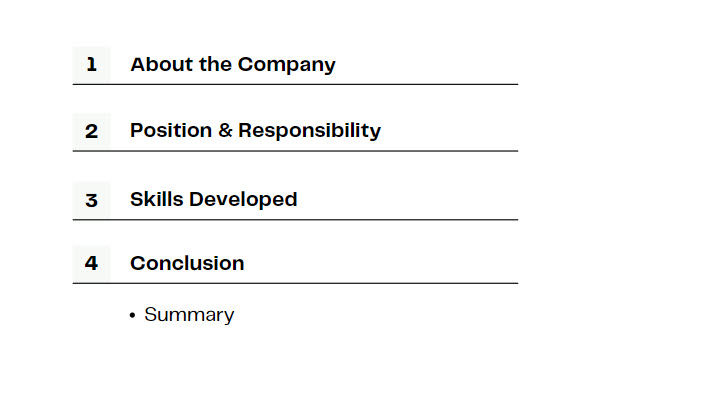
\includegraphics[width=400]{2023-05-11_18-46-53.jpg}
               \caption{Explains the flow of replication for Sentiment Analysis.}
        \end{figure}
        \newline
        \newline
         \break
    \end{itemize}

\end{frame}



%------------------------------------------------

%------------------------------------------------
% Sanjay Issues Explanation in details
%------------------------------------------------
\begin{frame}{Company Background}
    % Throughout your presentation, if you choose to use \section{} and \subsection{} commands, these will automatically be printed on this slide as an overview of your presentation
    \tableofcontents
%------------------------------------------------
%Overview
%------------------------------------------------

    \begin{columns}[c] % The "c" option specifies centered vertical alignment while the "t" option is used for top vertical alignment

        \column{.45\textwidth} % Left column and width
        \textbf{Service Provided}
        \begin{enumerate}
            \item truuth KYC.
            \item truuth Liveness.
            \item truuth Biopass.
        \end{enumerate}

        \column{.5\textwidth} % Right column and width
         Truuth is an organization founded to offer a digital identity service that is user-friendly, secure, and accurate it has products like Truth KYC that ensure a safe and seamless onboarding experience using AI and ML.

    \end{columns}   \\
    
\begin{table}[h!]
  \begin{center}
    \caption{An Overview of Truuth Company.}
    \label{tab:table1}
    \begin{tabular}{|l|c|r|} % <-- Alignments: 1st column left, 2nd middle and 3rd right, with vertical lines in between
      \hline
      \textbf{Headquarters } & \textbf{Company size} & \textbf{Founded}\\
      
      \hline
      Sydney & 20- 50  & 2009 \\
      \hline
     
    \end{tabular}
  \end{center}
\end{table}   \newline
\begin{itemize}
      
    \item \alert{Company Website:}\href{ https://www.truuth.id/}{ https://www.truuth.id}
 
    \end{itemize}
\end{frame}
%------------------------------------------------

%------------------------------------------------
% Dataset for the sentiment classification task}
%------------------------------------------------
\begin{frame}{Dataset for the sentiment classification task}
    \tableofcontents

    \textbf{Dataset}
    \begin{enumerate}
        \item Original IMDB  movie review dataset.\break 
            - Training set: 25,000 labeled and 50,000 unlabeled reviews.\break 
            - Test set: 25,000 labeled reviews.\break
            
         \item  Replication of 5\% the size of the original IMDB dataset.\break 
            - Training set: 1,111 labeled and 1,111 unlabeled reviews.\break 
            - Test set: 1,111 labeled reviews.\break
            
        \item Replication of new IMDB dataset.\break 
            - Training set: 1,000 labeled and 1,000 unlabeled reviews.\break 
            - Test set: 1,000 labeled reviews.\break
        \end{enumerate}
\end{frame}
%------------------------------------------------


%-------------------------------------------------------------

%------------------------------------------------


%------------------------------------------------
\begin{frame}{Evaluation Results}
    % Throughout your presentation, if you choose to use \section{} and \subsection{} commands, these will automatically be printed on this slide as an overview of your presentation
    \tableofcontents
%------------------------------------------------
%Overview
%------------------------------------------------

\begin{table}[h!]
    \begin{center}
    
    \caption{Summary of the accuracy scores of models on the IMDB sentiment classification task}
    \label{tab:table1}
    \begin{tabular}{|l|r|r|r|} % <-- Alignments: 1st column left, 2nd middle and 3rd right, with vertical lines in between
      \hline
      \textbf{Dataset} & \textbf{LM-LSTM} & \textbf{SA-LSTM} & \textbf{LSTM} \\
      \hline
      Original IMDB dataset (original work) & 92.36 & 92.76 & 86.5 \\
      5 \% of the original IMDB dataset & 57.6 & 56.8 & - \\
      New IMDB dataset & 50 & 50 & 50 \\
      \hline
    \end{tabular}
    
    \caption{Summary of the accuracy scores of models on the product classification task}
    \label{tab:table2}
    \begin{tabular}{|l|r|r|r|r|} 
      \hline
      \textbf{Dataset} & \textbf{LM-LSTM} & \textbf{SA-LSTM} & \textbf{LSTM} & \textbf{SVM}\\
      \hline
      Original DBpedia dataset (original work) & 98.5 & 97.66 & 86.36 & -\\
      2 \% of the original DBpedia dataset & 7.1 & 7.1 & 7.1 & - \\
      New Amazon dataset & 9.4 & 9.4 & 9.4 & 4.54\\
      \hline
    \end{tabular}
    \break
    \break
    \footnotesize{Pretraining: LM =  Language Model, and SA = Sequence Autoencoder}
  \end{center}
\end{table}

\end{frame}
%------------------------------------------------


%------------------------------------------------
% Findings and conclusion for the project
%------------------------------------------------
\begin{frame}{Conclusion/ Future Plans}
    \tableofcontents
%------------------------------------------------
%Overview
%------------------------------------------------

    \begin{columns}[c] % The "c" option specifies centered vertical alignment while the "t" option is used for top vertical alignment

        \column{.45\textwidth} % Left column and width
        \textbf{The Process}
        \begin{enumerate}
            \item Overall, Designed, build, and documented process to improve the Text format check...
            \item Overall, Designed, build, and improve the Visual Feature check.. 
        \end{enumerate}

        \column{.5\textwidth} % Right column and width
         Ensured the task text format/ visual feature check was implemented as per the requirement along with it the team was able to find and validate the code in the production system...

    \end{columns}   \\

\end{frame}
%------------------------------------------------



\end{document}